W tradycyjnym modelu opisującym biologiczne sieci neuronowe przyjmujemy, że jedyną wielkością fizyczną 
będącą nośnikiem informacji jest częstotliwość sygnału. Zatem skalarna wartość którą nazywamy wejściem
neuronu była zależna jedynie od częstotliwości sygnału wejściowego. 
Już w pierwszej chwili można zauważyć,
że model ten wiąże się z ogromną stratą informacji. 
Zapominamy o amplitudzie, przesunięciu sygnału, 
rozkładzie jego impulsów itd. 
W związku z tym, współcześnie są podejmowane próby analizy zależności między neuronami
w oparciu o model impulsowy. 
W modelu tym, nośnikiem informacji nie są częstotliwości sygnałów, 
ale położenie impulsów elektrycznych występujących w połączeniach między neuronami. 
W dalszym ciągu pomijamy inne szczegóły, takie jak kształt impulsu, czy też jego amplituda.
Warto w tym miejscu zwrócić uwagę, że na podstawie czasów występowania impulsów można obliczyć
częstotliwość sygnału, natomiast operacja odwrotna jest niemożliwa. 
Oznacza to, że model impulsowy jest bardziej szczegółowy do podejścia tradycyjnego.
Jednocześnie należy pamiętać, że ze względu na większą ilość przetwarzanych informacji podejście impulsowe wymaga zaangażowania 
znaczenie większych zasobów.

\section{Model impulsowy}
Jeżeli chcemy stworzyć dobry matematyczny opis zachowania neuronu, który będzie w przybliżeniu odpowiadał biologicznemu pierwowzorowi, 
musimy przyjąć następujące założenia:
\begin {itemize}
\item Jedno wejście - wiele wyjść
\item Prawdopodobieństwo “strzału” rośnie z czasem
\item Dynamika opisana przez conajmniej jedną zmienną
\end {itemize}
Pierwsze założenie jest oczywiste -- wiemy jak wyglądają neurony. 
Drugie założenie wynika z faktu, iż nie jest obserwowane w przyrodzie zjawisko neuronu ``milczącego''. 
Każdy neuron co jakiś czas wystawia na wyjście impuls. To zjawisko było jedną z podstaw do przyjęcia tradycyjnego modelu neuronowego.
Ostatnie założenie również jest względnie proste, skoro mówimy, że neurony wystawiają na wyjście impuls raz na jakiś czas, to musi być gdzieś
przechowywana informacja wynikająca z czasu ostatniego ``strzału'' oraz z czasów pojawiania się impulsów na wejściach. 
W pracy \cite{ponulak} zaproponowano następujący model:
    $$ C\frac{\mathrm{d}u}{\mathrm{d}t} (t) = -\frac1Ru(t)+\left(i_0(t) + \sum{w_ji_j(t)}\right)$$ 
gdzie: \\
    $u(t)$ -- zmienna stanu \\ 
    $C$ -- pojemność membrany \\
    $R$ -- rezystancja wejściowa\\
    $i_0(t)$ -- zewnętrzny prąd \\
    $i_j(t)$ -- wejście z $j$-tego połączenia synaptycznego\\
    $w_j$ -- waga $j$-tej synapsy

\section{Model sieci impulsowych}
Jeżeli opracowaliśmy już model pojedynczego neuronu, należy zastanowić się, jak może wyglądać model przechowywanie i przekazywania informacji
w sieci neuronów impulsowych.
\subsection{Czas najszybszej odpowiedzi}
W tym podejściu, informację przechowujemy wyłącznie jako czas dotarcia pierwszego impulsu do neuronu. 
Wydaje się, ze w tym podejściu tracimy dużą ilośc informacji, niemniej, zostało wykazane, że to podejście jest wystarzczające 
do poprawnego zakodowania u człowieka informacji dotyczących dotyku. 
Model został zwizualizowany na rys.~\ref{fig:TimeToFirstSpike}.
	\begin{figure}[ht]
		\centering
		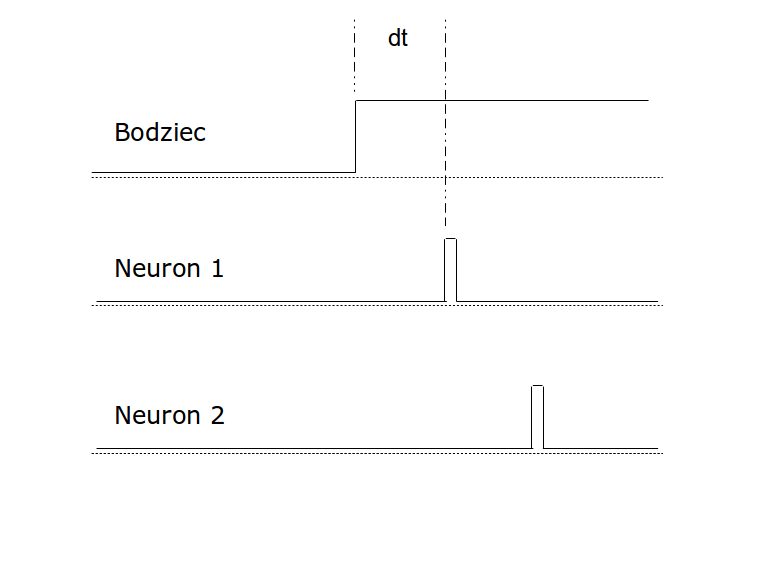
\includegraphics[width=\textwidth/2]{../TimeToFirstSpike.png}
		\caption{Czas najszybszej odpowiedzi}
                \label{fig:TimeToFirstSpike}
	\end{figure}
\subsection{Kodowanie kolejnością przybycia sygnałów}
To podejście wydaje sie być mniej stratne względem poprzedniego, aczkolwiek dalej zapominamy zupełnie o interwałach między impulsami.
Pewne badania wskazują jednak na skuteczność tego modelu w przypadku rozpoznawania statycznych obrazów.
Przykładowy przepływ informacji został pokazany na rys.~\ref{fig:ROC}.
	\begin{figure}[ht]
		\centering
		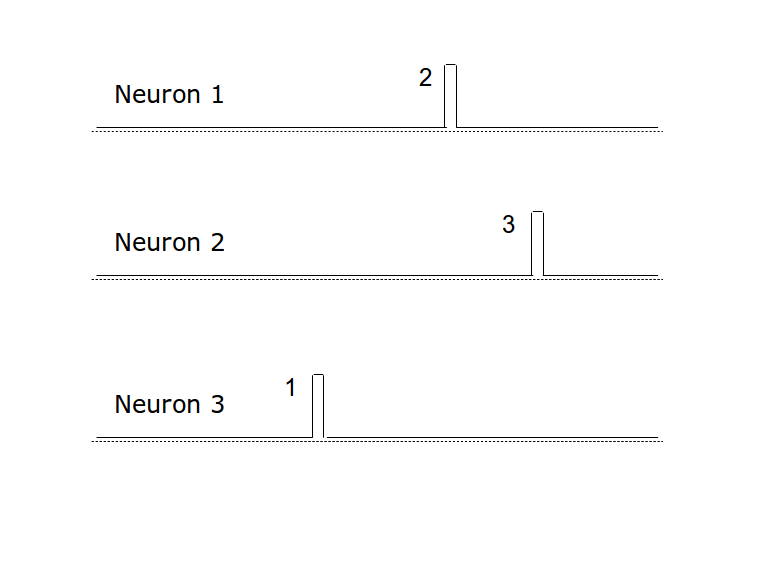
\includegraphics[width=\textwidth/2]{../ROC.png}
		\caption{Kodowanie kolejnością przybycia sygnałów}
                \label{fig:ROC}
	\end{figure}
\subsection{Względne opóźnienie impulsów}
W tym podejściu bierzemy pod uwagę interwały między impulsami, ale nie bierzemy pod uwagę, z którego neuronu wejściowego impulsy pochodziły.
Przykład informacji w tym modelu został przedstawiony na rys.~\ref{fig:Latency}.
	\begin{figure}[ht]
		\centering
		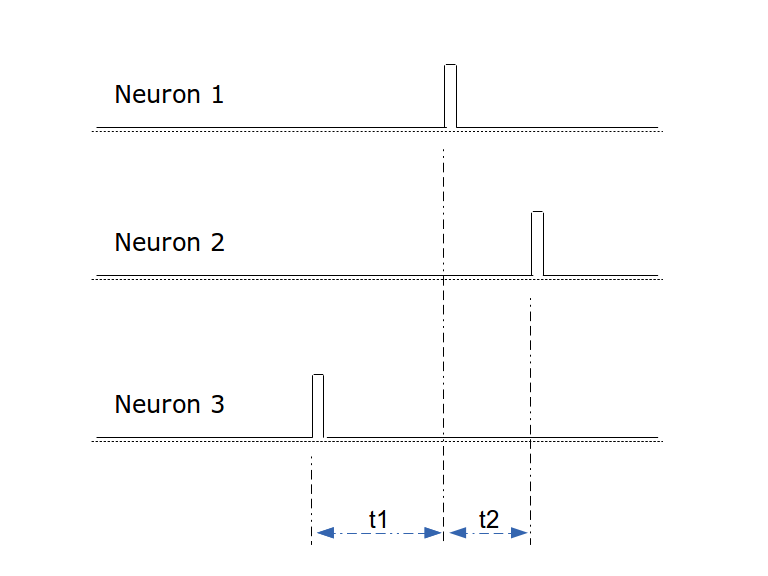
\includegraphics[width=\textwidth/2]{../Latency.png}
		\caption{Względne opóźnienie impulsów}
                \label{fig:Latency}
	\end{figure}
\subsection{Sieć rezonansowa}
W tym podejściu traktujemy neurony jako filtry, które reagują tylko na wybrane częstotliwości. 
Jeden neuron wejściowy przekazuje te same impulsy do kilku neuronów impulsowych. 
W zależności od ich częstotliwości, budzi się tylko jeden neuron. Zostało to zobrazowane na rys.~\ref{fig:ResonantBurst}
	\begin{figure}[ht]
		\centering
		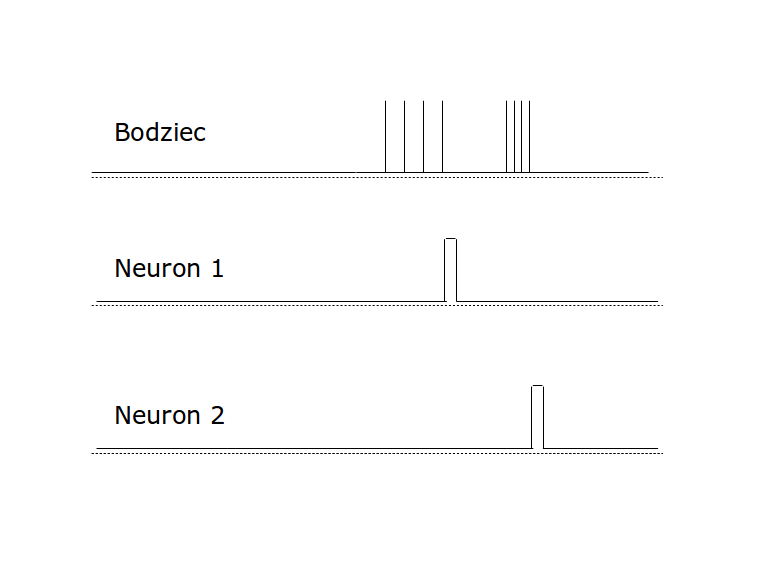
\includegraphics[width=\textwidth/2]{../ResonantBurst.png}
		\caption{Sieć rezonansowa}
                \label{fig:ResonantBurst}
	\end{figure}

\subsection{Kodowanie synchroniczne}
Wartość informacji zależy od tego, na których neuronach impuls pojawił się jednocześnie.
Z badań wynika, że niektóre neurony w ludzkim mózgu są wstanie synchronizować swoje impulsy z odchyleniem mniejszym od 1 ms.
Rys.~\ref{fig:CodingBySynchrony} ilustruje dwie różne wartości informacji w modelu synchronicznym.
	\begin{figure}[ht]
		\centering
		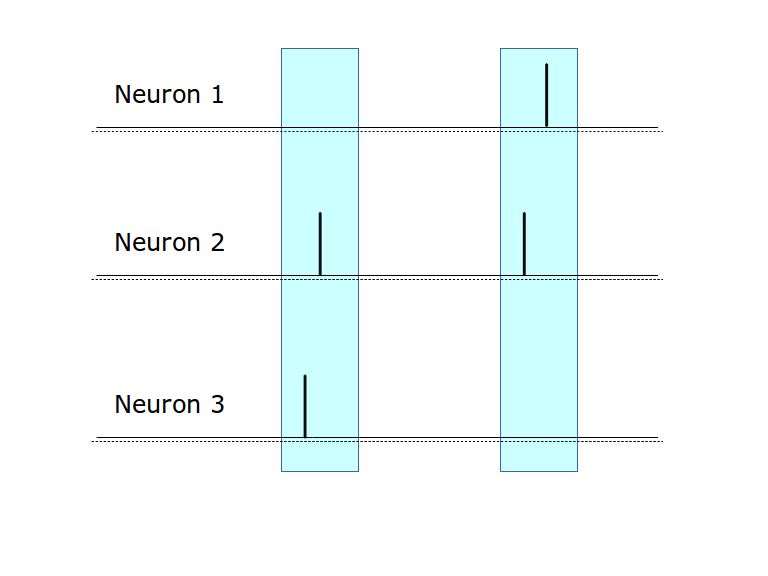
\includegraphics[width=\textwidth/2]{../CodingBySynchrony.png}
		\caption{Kodowanie synchroniczne}
                \label{fig:CodingBySynchrony}
	\end{figure}

\subsection{Kodowanie przez fazę}
W tym podejściu, najbardziej skomplikowanym, informacja zależy od tego, jaka sekwencja impulsów wystąpiła, 
kiedy sygnał referencyjny był w odpowiednim stanie. 
Na rys.~\ref{fig:Phase} przedstawiono takie kodowanie dwóch informacji przy sygnale referencyjnym prostokątnym, 
natomiast częściej stosuje się sygnal sinusoidalny.
	\begin{figure}[ht]
		\centering
		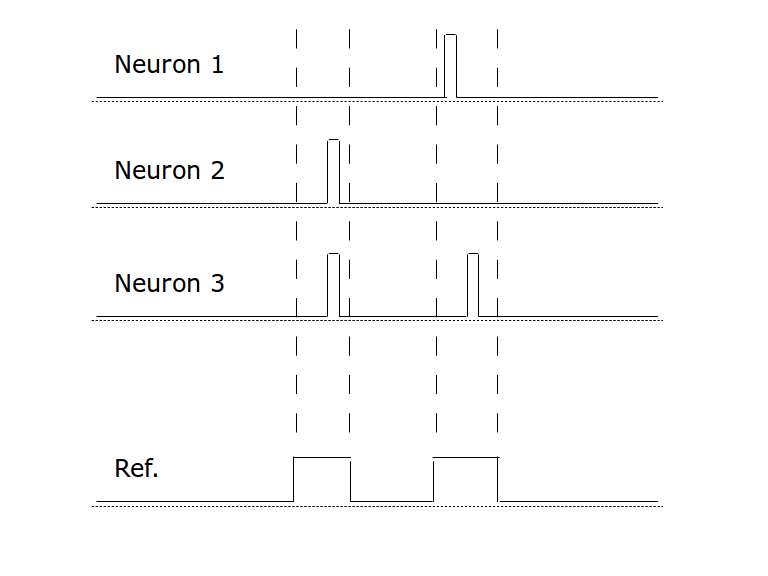
\includegraphics[width=\textwidth/2]{../Phase.png}
		\caption{Kodowanie przez fazę}
                \label{fig:Phase}
	\end{figure}
